% Created 2020-03-12 Do 13:42
% Intended LaTeX compiler: pdflatex
\documentclass[presentation]{beamer}
\usepackage[utf8]{inputenc}
\usepackage[T1]{fontenc}
\usepackage{graphicx}
\usepackage{grffile}
\usepackage{longtable}
\usepackage{wrapfig}
\usepackage{rotating}
\usepackage[normalem]{ulem}
\usepackage{amsmath}
\usepackage{textcomp}
\usepackage{amssymb}
\usepackage{capt-of}
\usepackage{hyperref}
\usetheme{default}
\author{DataColorado}
\date{\today}
\title{Presentation SFB-Farbig}
\hypersetup{
 pdfauthor={DataColorado},
 pdftitle={Presentation SFB-Farbig},
 pdfkeywords={},
 pdfsubject={},
 pdfcreator={Emacs 26.3 (Org mode 9.4)}, 
 pdflang={English}}
\begin{document}

\maketitle

\begin{frame}[label={sec:org7880101}]{Willkommen zur Präsentation}
\end{frame}
\begin{frame}[label={sec:org42d1de8}]{Präsentation der Software}
\end{frame}
\begin{frame}[label={sec:org781fa61}]{Reflektion}
\end{frame}
\begin{frame}[label={sec:orga42ae55}]{Team Kommunikation}
\begin{block}{Wahl der Kommunikationsplattform}
\end{block}
\end{frame}

\begin{frame}[label={sec:orgca97e8d}]{Lessons Learned}
\begin{block}{Löschen ist essentiell}
\end{block}
\begin{block}{Frame Works vor Implementierung}
Nicht eigene Implementierung sondern das Framework sollte das vorgehen im Front End bestimmten
\end{block}
\begin{block}{Primefaces for the WIN}
\end{block}
\end{frame}


\begin{frame}[label={sec:org3934d65}]{Aufwände über die einzelnen Projektphasen}
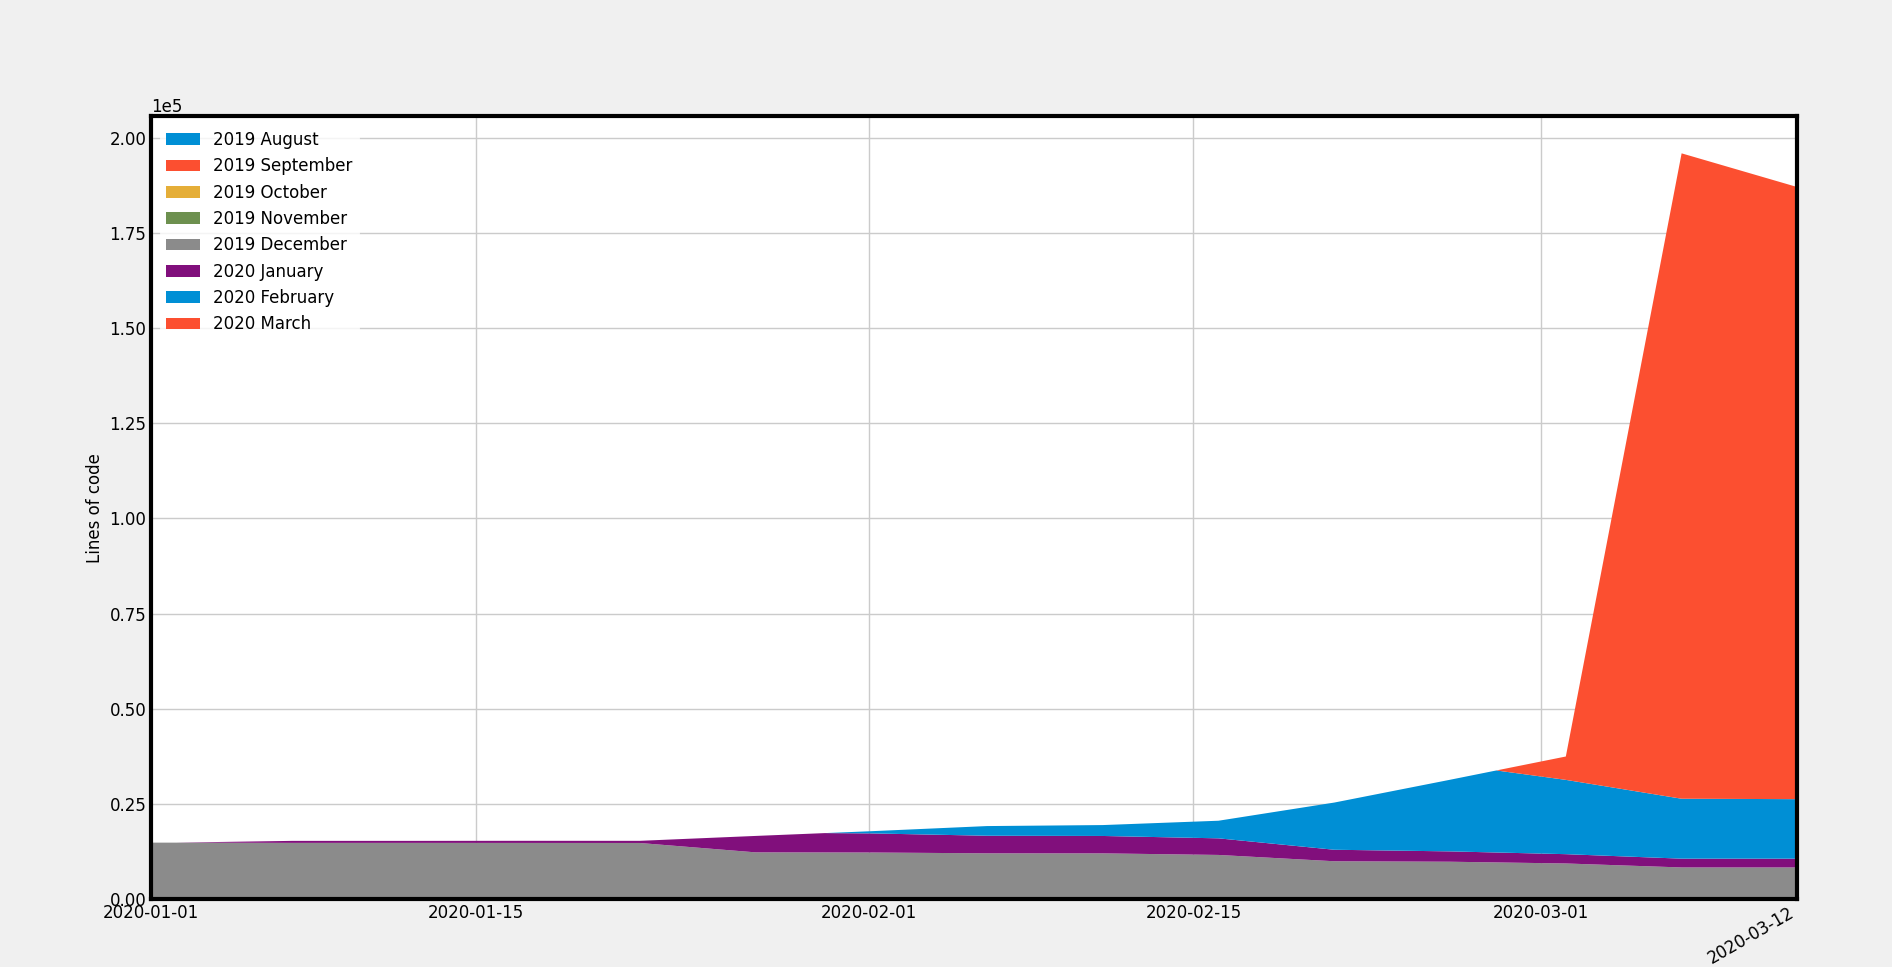
\includegraphics[width=1\textwidth]{project.png} 
\end{frame}

\begin{frame}[label={sec:org0b53452}]{Statistiken 1}
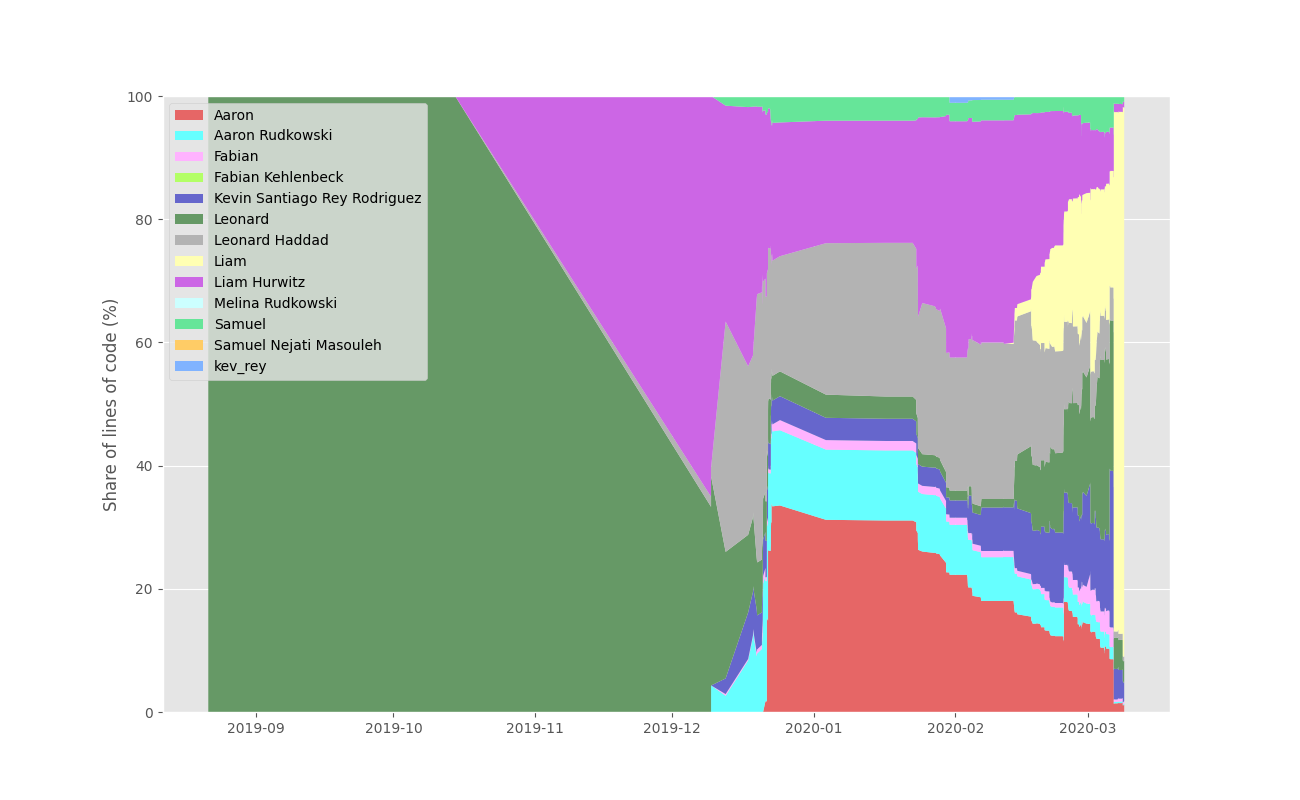
\includegraphics[width=1\textwidth]{stack.png}
\end{frame}

\begin{frame}{Statistiken 2}
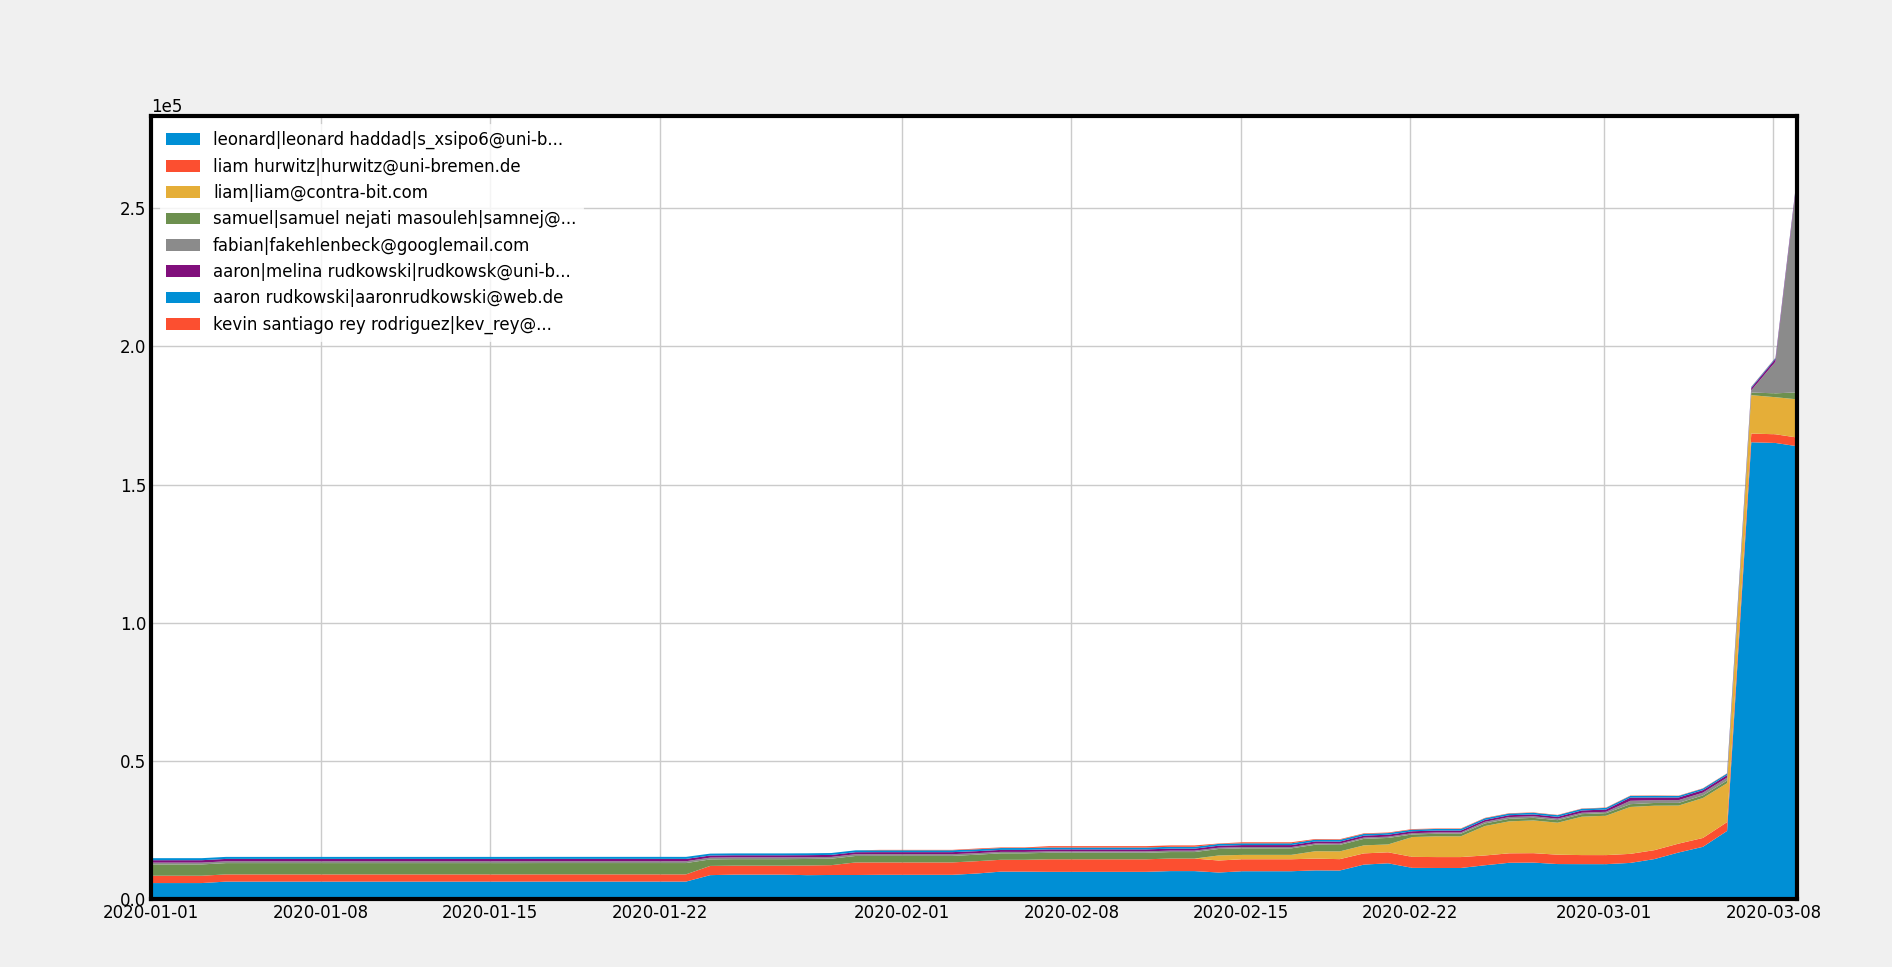
\includegraphics[width=1\textwidth]{ownership.png}  
\end{frame}

\begin{frame}{Erfahrung Auslandaufenthalt}
\end{frame}

\begin{frame}{Fragen über Fragen}
\end{frame}
\begin{frame}{Danke}
\end{frame}
\end{document}
